% !TEX encoding = UTF-8 Unicode
% !TEX root = ../report.tex
% 
\section{Análisis estadístico del algoritmo}
\label{analisis}

\subsection{Obtención de las muestras}
Para la \textbf{obtención de las muestras} necesarias para el \textbf{análisis estadístico} del algoritmo \texttt{HyperLogLog}
se ha utilizando un script programado en \textbf{\texttt{Ruby}}. Puede verse el código en el \textbf{apéndice \ref{codigo:ruby}}.

El script recibe como parámetros:
\begin{enumerate}
\item Los datasets de los que se quieren recoger muestras (por defecto \textbf{todos})
\item Los casos por muestra (por defecto \textbf{200})
\item Las memorias de las que recoger datos (por defecto \textbf{1024})
\item El directorio donde guardar resultados (por defecto \textbf{data})
\end{enumerate}

El script \textbf{compila y ejecuta el código en \texttt{C++} que implementa el algoritmo \texttt{HyperLogLog} para recoger los datos
y crea archivos con los resultados de cada muestra}, en forma de tabla. Finalmente, pregunta si se desean
\textbf{generar gráficas} a partir de los resultados obtenidos y, si se responde positivamente, ejecuta un \textbf{script en R que las genera autómaticamente} (disponible en el \textbf{apéndice \ref{codigo:graficas}}).

Para el primer análisis: \textbf{\nameref{analisis:mem_1024}}, las muestras se han obtenido utilizando los parámetros por defecto del script.

Para el segundo análisis: \textbf{\nameref{analisis:D1_mem}}, las muestras se han obtenido utilizando los parámetros:
\begin{description}
\item[Dataset] D1
\item[Memorias] 32, 64, 128, 256, 512, 1024, 2048, 4096, 8192, 16384
\end{description}

Y los otros parámetros con su valor por defecto.

\subsection{Memoria fijada a 1024 bytes}
\label{analisis:mem_1024}

En esta sección se estudia el comportamiento del algoritmo \texttt{HyperLogLog} en \textbf{9 \emph{datasets}} distintos limitando
la cantidad de memoria utilizada a \textbf{1024 bytes}. En el apéndice \ref{graficas} se incluyen gráficas que muestran los resultados
obtenidos para cada \emph{dataset} de forma detallada. Lo importante, sin embargo, es
\textbf{observar los resultados obtenidos de manera general para cada muestra}.

Se presentan las tablas \ref{tabla:resumen_1024} y \ref{tabla:count_1024} a modo de resumen para cada \emph{dataset}.

\begin{table}[h!]
    \centering
    \begin{tabular}{l r r r S S S}
    \strong{Dataset} & \strong{n} & \strong{N} & \strong{Est. media} &
    \strong{SE} & \textbf{T. medio ($ms$)} & \textbf{T. elem. ($\mu s$)}\\ \hline
    \newcounter{dataset}
\forloop{dataset}{1}{\value{dataset} < 10}{
\textbf{D\arabic{dataset}} &
\input{../data/D\arabic{dataset}/summary_1024.tex}
}
\end{tabular}
    \caption{Memoria fijada a 1024 bytes. Resumen de los resultados.}
    \label{tabla:resumen_1024}
\end{table}

\begin{table}[h!]
    \centering
    \begin{tabular}{l r r r r r r}
    \strong{Dataset} & \strong{[0, 1)} & \strong{[1, 5)} & \strong{[5, 10)} &
    \strong{[10, 15)} & \textbf{[15, 20)} & \textbf{[20, 100]} \\ \hline
\forloop{dataset}{1}{\value{dataset} < 10}{
\textbf{D\arabic{dataset}} &
\input{../data/D\arabic{dataset}/count_1024.tex}
}
\end{tabular}
    \caption{Memoria fijada a 1024 bytes. Clasificación de las ejecuciones según el error relativo (\%).}
    \label{tabla:count_1024}
\end{table}

Si se toma el \textbf{SE} de la tabla \ref{tabla:resumen_1024}, se puede observar que \textbf{no parece verse afectado por el \emph{dataset} utilizado}, puesto que en todos ellos oscila alrededor del $3\%$.

Por su parte, los \textbf{tiempos medios} sí que tienen un relación bastante obvia con \textbf{N:}
\textbf{cuanto mayor sea \textbf{N} más tardará el programa}. Esto es de esperar, puesto que el coste de un algoritmo suele
depender directamente de la entrada que recibe.

\textbf{Los tiempos por elemento varían considerablemente dependiendo del dataset}. Esto también es de esperar, puesto que
un dataset puede contener, en media, más elementos de \textbf{una longitud mayor} respecto a otro y, por lo tanto,
\textbf{aplicar la función de hash djb2 (sección \ref{implementacion:hash}) tendrá un coste mayor}.

Finalmente, en la tabla \ref{tabla:count_1024} se observa que los valores de \textbf{los errores relativos} están
concentrados, en todos los \emph{datasets}, en el intervalo $[0,5)$, con muy pocos valores en total por encima del $5\%$.
Este dato es muy positivo porque demuestra que el programa no precisa de muchas ejecuciones para dar una
estimación precisa, ya que cada ejecución tiene un \textbf{error relativo} razonablemente bajo. Por otro lado, este dato también
nos muestra que \textbf{la precisión del algoritmo para una ejecución en concreto no depende del \emph{dataset}}.

\subsection{Influencia de la memoria disponible}
\label{analisis:D1_mem}

Para estudiar el impacto de la \textbf{memoria disponible} en los resultados se ha usado el \textbf{\emph{dataset} D1},
con valores de memoria $m \in \{ 2^x \: | \; 5 \leq x \leq 14 \}$.

Se presentan las figuras \ref{figura:mem_estimation}, \ref{figura:mem_errors} y \ref{figura:mem_time} donde se puede observar la
\textbf{influencia de la memoria} sobre la \textbf{estimación media}, el \textbf{error estándar} y el \textbf{tiempo medio},
respectivamente.

\begin{figure}[h!]
    \centering
        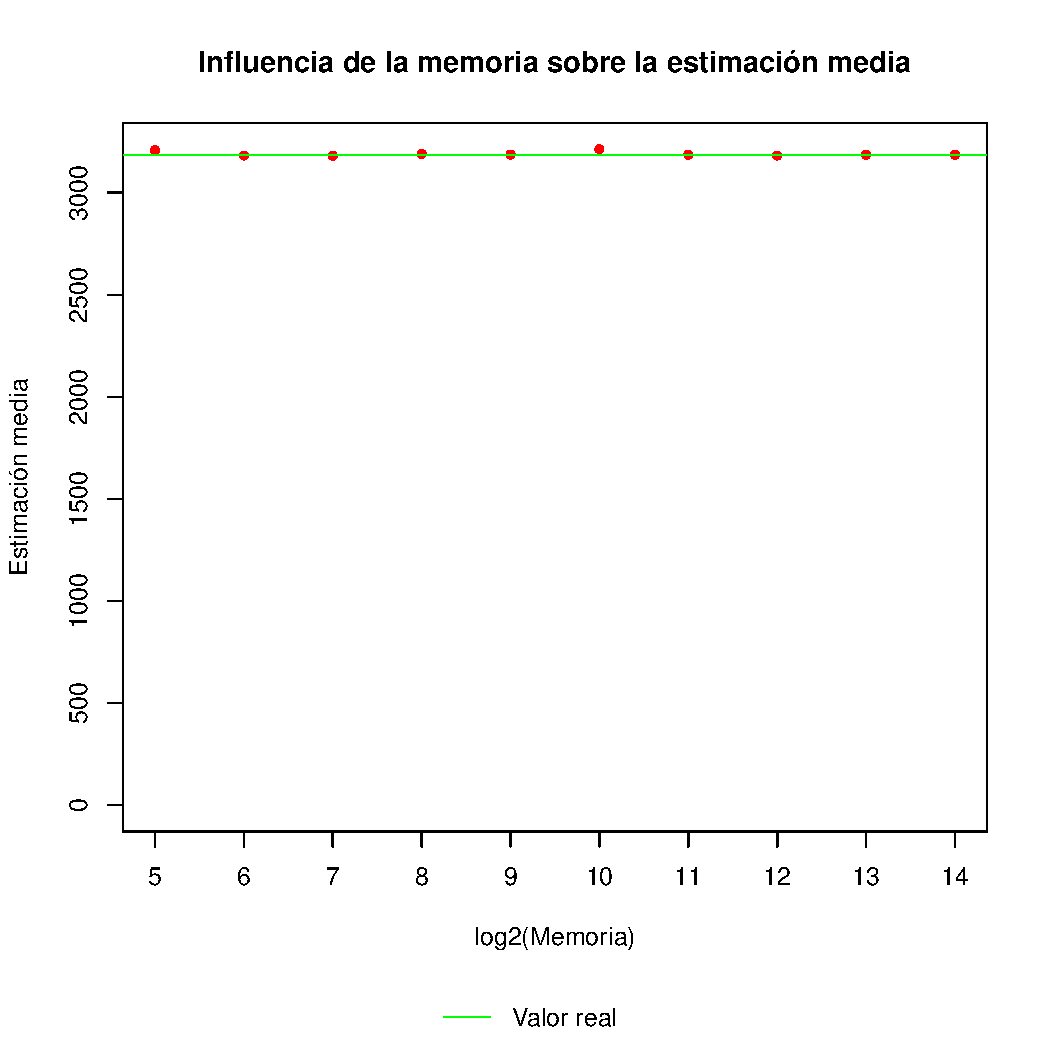
\includegraphics[width=0.64\textwidth]{../figs/D1/mem_estimation_rel.pdf}
        \caption{Influencia de la memoria disponible sobre la estimación media}
    \label{figura:mem_estimation}
\end{figure}

\begin{figure}[h!]
    \centering
        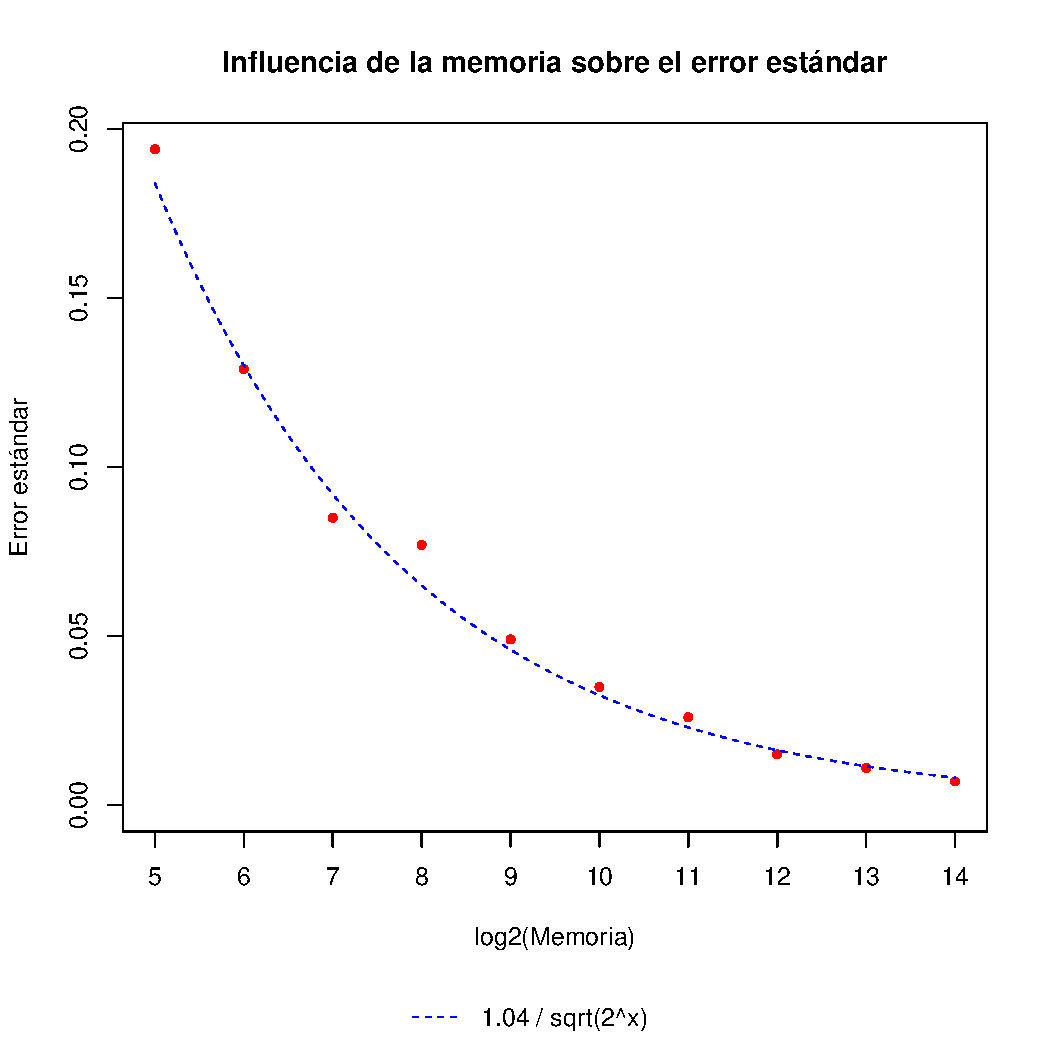
\includegraphics[width=0.64\textwidth]{../figs/D1/mem_errors_rel.pdf}
        \caption{Influencia de la memoria disponible sobre el error estándar}
    \label{figura:mem_errors}
\end{figure}

\clearpage

\begin{figure}[h!]
    \centering
        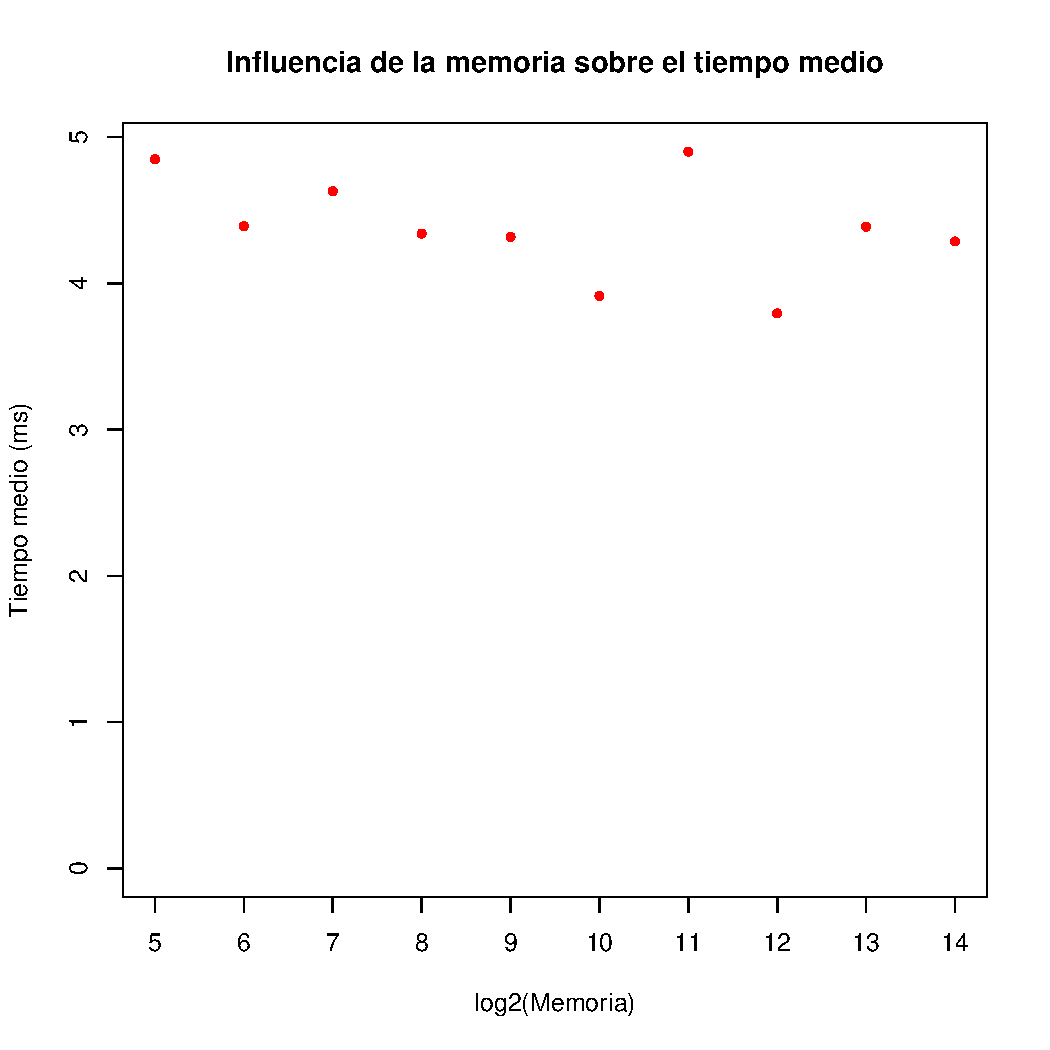
\includegraphics[width=0.64\textwidth]{../figs/D1/mem_time_rel.pdf}
        \caption{Influencia de la memoria disponible sobre el tiempo medio}
    \label{figura:mem_time}
\end{figure}

En la figura \ref{figura:mem_estimation} se observa que en todos los casos la estimación media es muy precisa. Esto podria llevar a
la conclusión \textbf{errónea} de que el tamaño de la memoria es irrelevante para el resultado final. No obstante, en la figura
\ref{figura:mem_errors} se observa que \textbf{cuanto mayor es la memoria usada menor es el \textbf{SE}}.
De hecho, puede observarse el \textbf{SE} disminuye considerablemente al principio, conforme la memoria aumenta. Sin embargo,
este efecto se suaviza rápidamente y \textbf{aumentar la memoria deja de ser efectivo}. Más exactamente, puede apreciarse como
\textbf{los distintos valores obtenidos obedecen perfectamente el error estándar esperado para el estimador de
\texttt{HyperLogLog}}:
$$SE = \frac{1.04}{\sqrt{m}}$$

\begin{table}[h!]
    \centering
    \begin{tabular}{l r r r S S S}
    \strong{Memoria (bytes)} & \strong{n} & \strong{N} & \strong{Est. media} &
    \strong{SE} & \textbf{T. medio ($ms$)} & \textbf{T. elem. ($\mu s$)}\\ \hline

\textbf{32} & 3185 & 17219 & 3209 & 0.194 & 4.849 & 0.282\\ \hline

\textbf{64} & 3185 & 17219 & 3182 & 0.129 & 4.392 & 0.255\\ \hline

\textbf{128} & 3185 & 17219 & 3181 & 0.085 & 4.631 & 0.269\\ \hline

\textbf{256} & 3185 & 17219 & 3190 & 0.077 & 4.341 & 0.252\\ \hline

\textbf{512} & 3185 & 17219 & 3187 & 0.049 & 4.319 & 0.251\\ \hline

\textbf{1024} & 3185 & 17219 & 3210 & 0.027 & 4.850 & 0.282\\ \hline

\textbf{2048} & 3185 & 17219 & 3186 & 0.026 & 4.901 & 0.285\\ \hline

\textbf{4096} & 3185 & 17219 & 3182 & 0.015 & 3.795 & 0.220\\ \hline

\textbf{8192} & 3185 & 17219 & 3186 & 0.024 & 4.420 & 0.257\\ \hline

\textbf{16384} & 3185 & 17219 & 3186 & 0.007 & 4.287 & 0.249\\ \hline


\end{tabular}
    \caption{Influencia de la memoria sobre el dataset D1. Resumen de resultados.}
    \label{tabla:resumen_mem}
\end{table}

\begin{table}[h!]
    \centering
    \begin{tabular}{l r r r r r r}
    \strong{Memoria} & \strong{[0, 1)} & \strong{[1, 5)} & \strong{[5, 10)} &
    \strong{[10, 15)} & \textbf{[15, 20)} & \textbf{[20, 100]} \\ \hline

\textbf{32} & 9 & 27 & 43 & 40 & 25 & 56\\ \hline

\textbf{64} & 9 & 40 & 59 & 46 & 28 & 18\\ \hline

\textbf{128} & 13 & 81 & 60 & 31 & 10 & 5\\ \hline

\textbf{256} & 23 & 74 & 70 & 28 & 2 & 3\\ \hline

\textbf{512} & 26 & 126 & 45 & 3 & 0 & 0\\ \hline

\textbf{1024} & 62 & 122 & 16 & 0 & 0 & 0\\ \hline

\textbf{2048} & 70 & 127 & 3 & 0 & 0 & 0\\ \hline

\textbf{4096} & 106 & 94 & 0 & 0 & 0 & 0\\ \hline

\textbf{8192} & 146 & 54 & 0 & 0 & 0 & 0\\ \hline

\textbf{16384} & 186 & 14 & 0 & 0 & 0 & 0\\ \hline


\end{tabular}
    \caption{Influencia de la memoria sobre el dataset D1. Clasificación de las ejecuciones según el error relativo (\%).}
    \label{tabla:count_mem}
\end{table}

Si se analiza la tabla \ref{tabla:count_mem} se puede apreciar que los
\textbf{errores relativos} de las ejecuciones con memorias más reducidas se concentran en los valores superiores al $10\%$. No es
hasta que la \textbf{memoria disponible} aumenta hasta los 512 bytes que el \textbf{error relativo} se concentra por debajo del
$10\%$, y solo a partir de los 4 Kbytes dejan de aparecer ejecuciones por encima del $5\%$. Por tanto, para obtener una estimación
precisa con poca memoria sería necesario \textbf{realizar diversas ejecuciones}, aumentando así el tiempo total, tal vez más de lo
posible.

En general se podría concluir que el mínimo de \textbf{memoria necesaria} es de unos 512 bytes, ya que su \textbf{SE} es del $5\%$
aproximadamente, un valor aceptable en la mayoría de casos. Por otro lado, dependiendo de la importancia de la precisión, se puede
aumentar o disminuir este valor.
